\chapter{Skin Lesion Diagnosis}
\label{chapter:sota}

This chapter provides an overlook into the state-of-the-art applications and methods used to diagnose skin lesions, including hand-crafted image processing techniques and recent end-to-end deep learning approaches. In order to provide some context, \Cref{section:ehealth_mhealth} reviews the literature related to dermatology applications for the self-surveillance of skin lesions. Section \ref{section:hand-crafted} presents an exploratory view into different handcrafted computer vision methods for skin lesion diagnosis. Section \ref{section:skin_deep_learning} focuses on end-to-end approaches for skin lesion classification that use deep learning methods. Finally, \Cref{section:limitations} identifies some of the limitations and opportunities of deep learning methods towards skin lesion diagnosis.

\section{eHealth and mHealth Applications}
\label{section:ehealth_mhealth}
    Online health, eHealth, and mHealth applications represent a rapidly developing field of medicine that has the potential to become a powerful tool in the diagnosis and management of skin diseases \cite{Jaworek-Korjakowska2018}. These applications aim to enhance clinical care, promote health, prevent diseases, and most importantly provide medical support when it is not available at a particular location or time. \par
    
    Currently, several production-ready skin lesion classification systems are available for both skin professionals and patients wishing to self monitor their skin. Kassianos \textit{et al.} \cite{Kassianos2015} reviewed mHealth applications for the detection of melanoma targeted at the general community, patients, and clinicians. The authors reported the existence of 39 dermatology-related applications available on the market, in July 2014, in a range of functionalities including information, education, classification, risk assessment, and monitoring change. Over half of them provided information, advice, or education about melanoma, ultraviolet radiation exposure prevention advice, and skin self-examination strategies, mainly using the ABCDE (A, Asymmetry; B, Border; C, Colour; D, Diameter; E, Evolving) method \cite{Nachbar1994}. Half of the apps helped users take and store images of their skin lesions either for review by a dermatologist or for self-monitoring to identify change, an important predictor of melanoma. A similar number of apps provide reminders to help users monitor their skin lesions. A few apps offered an expert review of images. Four apps provided a risk assessment to patients about the probability that a lesion was malignant or benign, and one app calculated users’ future risk of melanoma. There was little evidence of clinical or research-based input into the design of these apps. Furthermore, none of the apps appeared to have been validated for diagnostic accuracy using established research methods. \par
    
    More recently, Zaidan \textit{et al.} \cite{Zaidan2018} reviewed the literature on mHealth for skin cancer diagnosis in the period from 2011 to 2016. A total of 89 articles were classified into four groups: development and design, analytical, evaluative and comparative, and review and survey studies. Out of the 89 articles, 43 focus on the development of various AI algorithms and applications for assisting in the prevention and early detection of malignant melanoma. A total of 20 articles involve analytical studies on the incidence of skin cancer, the classification of malign cancer or benign cancer, and methods for prevention and diagnosis. A total of 15 articles consist of studies that range from evaluation or comparison of mobile apps to the exploration of features designed for skin cancer detection. A total of 11 articles comprise reviews and surveys referring to actual applications or providing a general overview of the technology. \par
    
    In the same year, Jaworek-Korjakowska and Kleczek \cite{Jaworek-Korjakowska2018} reported the existence of about 45 mobile applications related to mole diagnosis available on Apple’s App Store in March 2017. Most of them offered only educational information on melanoma, nearly half of them allowed the user to take photos of their moles and track changes over time using simple visual comparison, and only four applications performed melanoma risk assessment or lesion classification based on image analysis. These applications are DermaCompare (risk assessment through image matching), Lūbax (mole diagnosis through content-based image retrieval), MySkinApp (risk assessment), and SkinVision (risk assessment through fractal analysis). SkinVision in particular classifies lesions as either low, medium or high risk of skin cancer by using a risk assessment algorithm based on gray-scale images of lesions and their associated fractal maps. It achieves an overall sensitivity of 73\%, a specificity of 83\%, and an accuracy of 81\%. The positive and negative predictive values were 49\% and 83\%, respectively \cite{Jaworek-Korjakowska2018}.
    
    As an alternative, some web applications help dermatologists at the diagnosis of skin lesions, such as Metaoptima's Dermengine web application \cite{dermengine}. Their Visual Search tool compares user-submitted images with similar images in a database of thousands of pathology-labeled images gathered from other dermatologists, based on visual features such as the color, shape, or patterns of a lesion \cite{dermengine}. \par
    
    Unfortunately, from the presented eHealth applications, only two were certified by authorities, namely, SkinVision which received the European “CE” Marking and DermaCompare that was approved by the U.S. Food and Drug Administration \cite{Jaworek-Korjakowska2018}. This highlights larger concerns with these types of applications, namely, the lack of the required performance for medical-grade applications and the false advertising of these systems performance. This is corroborated by reports such as the one done by Maier \textit{et al.} for the Journal of the European Academy of Dermatology and Venerology, which shows that there is a lack of accuracy within mHealth apps such as SkinVision on tasks like melanoma detection \cite{Maier2015}. Other incidents also reflect this concern, such as in 2015 the Federal Trade Commission in the U.S., filing cases against several skin mole evaluation applications for false advertising of their capabilities to detect skin cancers \cite{ftc}. \par

\section{Hand-crafted Image Processing Methods}
\label{section:hand-crafted}
    As seen in the previous section, some of the skin lesion classification eHealth/mHealth applications used hand-crafted image processing methods in order to make assessments (\textit{e.g.}, ABCDE method). Typically, to classify a skin lesion from dermoscopic images using handcrafted features, one must first segment the lesion, then extract relevant features from the segmented part of the image, and finally, classify the lesion into a specific class \cite{Pathan2018}. Different approaches for each of these tasks will be presented. \par
    
    \subsection{Lesion Segmentation}
    Skin lesions can be distinguished from the surrounding area of the skin due to their color, intensity, and texture. Lesion segmentation aims to separate that region from the rest of the image so that further processing can be applied (\textit{e.g.}, identification of global morphological features specific to the lesion, and segmentation of various local features at a later stage). This can become a challenging problem because dermoscopic images often come with various artifacts (\textit{e.g.}, hairs, ruler marks, date markers, ink, bubbles), and in many cases, there is a low-contrast between the bounded region and the surrounding area (\textit{e.g.}, lighting conditions, skin tone variations). Additionally, the lesion itself can have variations in color, texture, shape, size, and location that make it difficult to contrast it with the background. Although the impact of these factors can be minimized with proper pre-processing. \par
    
    Therefore, both high- and low-level methods for performing lesion segmentation have been proposed over the years. Histogram thresholding is one simple example used by some authors like Celebi \textit{et al.} \cite{EmreCelebi2013}, which segments image regions based on whether pixels from that region are below a specific pixel intensity or not. Edge detection is another simple technique used \cite{Abbas2011} in which lesions are segmented based on discontinuities. However more complex approaches like clustering \cite{Mete2011}, active contours \cite{Zhou2013}, graph theory \cite{Yuan2009} and probabilistic modeling \cite{Wong2011} can also be found in the literature. \par
    
    \subsection{Feature Extraction}
    With the bounded region, one can start feature extraction by identifying points of interest within that region. Such interest points can be attributes such as color, texture, shape, structure, relative size, and location of the lesion \cite{Barata2014}. As a result of several studies, multiple algorithms have been identified to help determine whether a given skin lesion is melanocytic/nonmelanocytic and benign/malignant, namely: 
    \begin{itemize}
        \item Pattern analysis \cite{Pehamberger1987}\cite{Barzegari2005} identifies melanocytic lesions using local and global patterns. Local patterns include pigment system, dabs and globules, streaks, blue whitish shroud, relapse structures, hypopigmentation, and vascular structures. Global patterns include reticular, globular, cobblestone, homogeneous, stardust, parallel, multi-component, lacunar, and unspecific patterns;
        
        \item ABCD-rule \cite{Nachbar1994} evaluates melanoma diagnosis using four criteria which include asymmetry, border irregularity, color, and diameter. Each criterion is multiplied by a weight factor to establish a \ac{TDS}. A lesion is classified as benign if its \ac{TDS} score is less than 4.75, if it is within the 4.75 and 5.45 range, it is considered as a possible melanoma, and finally if the \ac{TDS} is above 5.45 it is likely a melanoma;
        
        \item Menzies method \cite{Johr2002} is based on a set of negative and positive features. Negative features include patterns that are point or axial asymmetric and presence of a solitary shading (gray, ebony, blue. red, tan, and dark brown). The nine positive features are radial streamings, multiple brown dots, blue white veils, pseudopods, peripheral ebony globules, depigmentations, multiple hues, numerous blue or dark spots, and finally expanded networks. For a lesion to be classified as melanoma at least one positive feature must be found;
        
        \item 7-point checklist \cite{Unlu2014}\cite{Walter2013} assigns a score based on three major (atypical pigment network, blue-white veil, and atypical vascular pattern) and four minor criteria (irregular streaks, irregular pigmentation, irregular dots/globules, and regression structures). To score a lesion, the proximity of a major criterion is given 2 points and that of a minor model is given 1 point. The lesion is named as melanoma when the aggregate score is more prominent than or equivalent to 3;
        
        \item CASH algorithm \cite{Henning2007} is designed as a simplified form of pattern analysis in which lesions are evaluated according to the color, architecture, symmetry, and homogeneity.
    \end{itemize}
    
    A comparison of these algorithms reveals two diverging approaches to simplified melanoma detection. The ABCD rule and CASH mainly quantify the overall organization of a lesion by assessing features such as symmetry, architectural disorder, border sharpness and heterogeneity in colors and structures. The 7-point checklist relies on the identification of atypical appearances of dermoscopic structures (\textit{e.g.}, atypical network) in distinction from otherwise normal counterparts or on identifying unique structures strongly associated with melanoma. The Menzies method includes elements of both approaches. Although each algorithm has unique criteria, there is significant overlap in their concepts. \par
    
    \subsection{Disease Classification}
    Finally, the image features extracted can be fed to a classifier that should be able to distinguish between different types of lesions (\textit{e.g.}, melanomas from benign lesions). Such classifiers can be based on a multitude of algorithms such as artificial neural networks or support vector machines. Figure \ref{fig:classificationalgorithms} illustrates the distribution of the most used algorithms for classifying features from skin lesions as presented by Prabhu \textit{et al.} \cite{Pathan2018}. \par
    
    While these types of approaches provide a way of classifying skin lesions, they require domain knowledge, particularly, when performing segmentation and feature extraction. More recently, deep learning techniques have become prominent in fields such as medical imaging, and more specifically in skin lesion diagnosis, as seen by some surveys \cite{Hu2018} \cite{Litjens2017}. In contrast with hand-crafted methods, deep learning can be used without requiring preliminary steps such as lesion segmentation or feature extraction. \par
    
    \begin{figure}[ht]
      \centering
        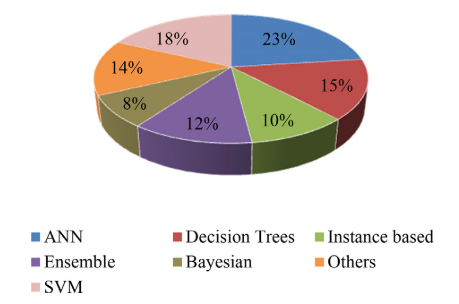
\includegraphics[width=0.5\linewidth]{figs/classificationalgorithms.png}
      \caption{Contribution of each classification method to the total number of dermoscopic studies according to the review paper of Prabhu \textit{et al.} \cite{Pathan2018}.}
      \label{fig:classificationalgorithms}
    \end{figure}

\section{Deep Learning for End-to-end Classification of Skin Lesions}
\label{section:skin_deep_learning}
    Deep learning refers to computational models composed of multiple processing layers capable of learning representations of data with multiple levels of abstraction \cite{Goodfellow-et-al-2016}. The initial impact of deep learning for medical imaging was revealed through a special issue published in 2016 at the IEEE Transactions on Medical Imaging \cite{Greenspan2016}. It explains the principles and methods of deep learning applied to medical image analysis. These structures can be found in approaches to medical imaging problems such as organ segmentation, lesion detection, and tumor classification. \par
    
    Recently, deep neural networks appear as state-of-the-art solutions for medical imaging problems due to advancements in the field \cite{Litjens2017}. These advancements include the research and development of new methods to prevent overfitting, the rise of computational power along with the use of graphical processing units, and lastly, the development of high-level modules such as Tensorflow\footnote{\url{https://www.tensorflow.org/}} \cite{Abadi} that help train and test neural networks. \par    
    
    One key advantage of deep learning over other machine learning algorithms is that it removes the need for feature engineering, a process that requires knowledge expertise of the problem domain but can be time-consuming and introduce human error if not all the algorithm details are described (\textit{i.e.}, edge cases). Another key advantage of deep neural networks is that these models scale well with the amount of data available, as opposed to other machine learning methods in which performance stagnates past a certain amount of samples \cite{Alom2019}. \par 
    
\subsection{Transfer Learning Approaches}
\label{section:skin_transfer_learning}
    Perhaps one of the most popular approaches for skin cancer classification using deep \ac{CNN}s, was published in 2017 by Esteva \textit{et al.} \cite{Esteva2017}, in which their classifier could diagnose keratinocyte and melanoma cancer. Their dataset combines biopsy-proven data from the \ac{ISIC} archive, Edinburgh Dermofit Library, and the Stanford Hospital, totaling an astonishing 129450 samples which remains one of the biggest efforts in data collection in the area. This dataset was also oversampled using data augmentation with flips, rotations, and crops. The authors follow a transfer learning approach by leveraging the weights of the InceptionV3 \cite{inceptionv3} network pre-trained on ImageNet \cite{Deng2010}, on top of which they replaced the classifier. Afterward, they measured the network's performance by pitting it against 21 dermatologists on biopsy-proven samples. Finally, the presented results proved that their classifier had comparable performance to that of those board-certified dermatologists with an \ac{AUC} of 0.94.\par
    
    Haenssle \textit{et al.} \cite{Haenssle2018} presented a very similar approach to Esteva \textit{et al.} \cite{Esteva2017}. They also fine-tuned the InceptionV3 pre-trained model \cite{inceptionv3}, but the analysis was limited to samples of melanoma and benign nevi. Similarly to Esteva \textit{et al.}, they compared their approach with 58 dermatologists, which at the time was the largest number of dermatologists involved in a publication about automated skin lesion classification \cite{Brinker2018}. They achieved \ac{AUC} of 0.86, which is a considerably lower score than that of Esteva \textit{et al.}. \par
    
    More recently, Tschandl \textit{et al.} \cite{Tschandl2019} also compared the performance of 95 human raters with different experience in dermoscopy (all medical personnel, from which 62 board-certified dermatologists):
    \begin{itemize}
        \item Their approach employed a combined \ac{CNN} trained on 13724 samples of lesions (7895 dermoscopic and 5829 close-ups) and tested on 2072 samples. These samples are part of 8 different lesion classes, namely, actinic keratoses and intraepithelial carcinoma (also known as Bowen disease), basal cell carcinoma (all subtypes), benign keratosis-like lesions (including solar lentigo, seborrheic keratosis, and lichen planus–like keratosis), dermatofibroma, melanoma, invasive squamous cell carcinoma and keratoacanthoma, benign sebaceous neoplasms, and benign hair follicle tumors;
        \item The combined \ac{CNN} is composed of two distinct pre-trained models, namely the InceptionV3 \cite{inceptionv3} model and the ResNet50 model \cite{resnet} pre-trained on ImageNet;
        \item Human raters were compared to the combined \ac{CNN} based on the \ac{AUC} metric calculated from 50 cases drawn randomly from the entire test set. Furthermore, human raters were divided into three groups of experience, namely, beginners, intermediates, and experts.
        \item Results showed that the combined \ac{CNN} was able to diagnose lesions as accurately as human experts (0.733 vs 0.741), and outperform both beginner and intermediate experienced raters. 
        \item Although these results are promising, the authors pointed that the evaluation metrics used to measure diagnostic performance might not represent the performance in a real-world scenario, because it does not take into account the potential loss of life-years and apply penalties to misdiagnoses of more aggressive disease. 
        \item Lastly, the authors highlighted the importance of the dataset used to train these models and affirmed that future efforts should be put into making larger amounts of samples of common and rare lesions available to the research community, such that future approaches can increase performance.
    \end{itemize}
    
    For general image recognition problems, datasets such as ImageNet \cite{Deng2010} which contains over 14 Million samples with over 20000 classes serve as a benchmark. However, for skin lesion diagnosis systems, it is difficult and in many times impossible to compare the performance of published classification results since many authors use nonpublic datasets for training and testing \cite{Brinker2018}. \par
    
    However, some attempts have been made to address this problem. For example, the publicly available \ac{HAM10000} dataset \cite{ham10000} which consists of 10015 dermatoscopic images. It contains classes such as melanoma, melanocytic nevi, actinic keratoses, intraepithelial carcinoma, Bowen's disease, basal cell carcinoma, benign keratosis, dermatofibroma, and finally vascular lesions. Furthermore, organizations such as \ac{ISIC} provide an open-source public access archive of skin images, called \ac{ISIC} archive \cite{archive}. It can be used for the development or testing of automated skin lesion diagnosis systems \cite{isic2019}. This organization also places a challenge every year which serves as a benchmark for skin lesion classification systems. \par
    
    \subsubsection{International Skin Imaging Collaboration Challenge 2018}

    Automated skin lesion classification systems should not only provide information and treatment options, but also detect skin cancer cases with reasonable sensitivity and specificity \cite{isic2018}. While the first goal is a multi-class problem (diagnosis out of range of classes), the second is a binary one ("biopsy" or "no biopsy"). In third task of the \ac{ISIC} 2018 challenge, participants were asked to develop a multi-class classifier to distinguish between 7 different types of skin lesions. The provided dataset include lesion samples of melanocytic nevus, melanomas, basal cell carcinomas, actinic keratosis, benign keratosis, dermatofibromas, and finally vascular lesions. Participants were ranked based on the \ac{BMA} as it is closer to real evaluation of a dermatologist \cite{isic2018}, but other metrics such as accuracy or \ac{AUC} are computed for scientific completeness (see \Cref{section:metrics}). \par 
    
    The top 3 submissions had \ac{BMA}s of 88.5\%, 88.2\%, 87.1\%, respectively, and were all submitted by Aleksey Nozdryn-Plotnicki and Yolland \cite{isic2018top3}, which were part of a team at Metaoptima (the company behind Dermengine \cite{dermengine}). To train those models they used the provided dataset, plus samples from the \ac{ISIC} archive and samples from a proprietary dataset. All samples were preprocessed by normalizing them with the shades of gray method \cite{shadesgray}. Additionally, they augmented the training data by performing random horizontal flips, random rotations, changes in brightness, saturation, and contrast. They employed a transfer learning approach using several models pre-trained on ImageNet (\textit{e.g.}, InceptionV3 or ResNet) and then ensembled the models with the highest accuracy \cite{isic2018top3}. \par
    
    Furthermore, some submissions presented interesting ways to improve the results without the need for external data. More specifically: 
    \begin{itemize}
        \item Gessert et at. \cite{gessert2018} performed an extensive hyperparameter tuning with different optimization algorithms, in which they concluded that the Adam optimizer \cite{adam} was the best choice. They also have a particularly interesting approach for inference (shown in \autoref{fig:gessert2018}), while performing competitively with an \ac{BMA} of 0.83 (fourth place). They ensembled different pre-trained models, namely, SENet154, ResNeXt101, Densenet201, Densenet161, Densenet169, SE-Resnet101, and PolyNet. For each architecture 6 models are trained, 5 by performing 5-fold cross-validation and 1 by training it with the whole dataset (without validation set). Evaluation is performed by cropping 36 patches from each test sample and feeding those patches to each model. Then, for the models that do not have a validation set, the softmax probabilities are averaged across all 36 patches. For cross-validated models, predictions are combined using a \ac{SVM}. Finally, both results are combined by averaging the softmax probabilities;
        \begin{figure}[ht]
            \centering
            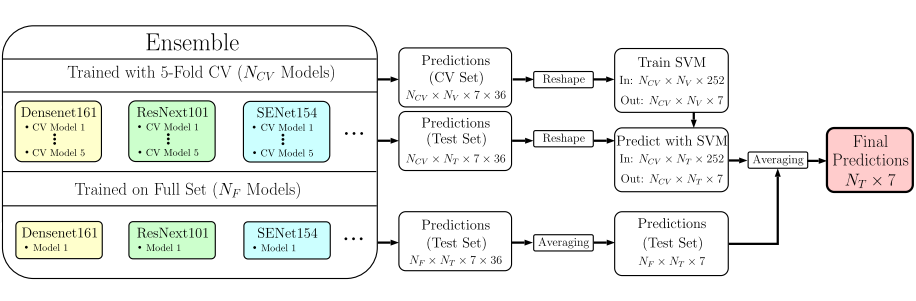
\includegraphics[width=\linewidth]{figs/gessert2018.png}
            \caption{The evaluation strategy for the generation of final predictions of Gessert \textit{et al.} \cite{gessert2018}.}
            \label{fig:gessert2018}
        \end{figure}
        
        \item Ashraful Alam Milton \cite{Milton2018} followed an approach based on transfer learning from models of PNASNet-5-Large, InceptionResNetV2, SENet154, InceptionV4 trained on ImageNet. He interestingly noted that in the first few epochs the gradient is very erratic. Thus, he presented an approach in which during the first 2 epochs only the classifier is trained with the convolutional base frozen in order to avoid updating weights towards the wrong direction. Finally, his approach achieved a \ac{BMA} of 0.76 on the validation set;
        
        \item Bissoto \textit{et al.} \cite{Bissoto2018} (who won 3rd place in the 2017 edition) transferred knowledge from models of InceptionV4, ResNet-152, and DenseNet-161 trained on ImageNet, by training with online data augmentation (\textit{e.g.}, random crops, flips, rotations, shears, color transformations), SGD with the learning rate being decreased by a factor of 10 whenever validation loss didn’t improve for 10 epochs, eventually building an average of 15 models trained only with the challenge data that attained a score of 0.803.
    \end{itemize}
    
    Tschandl \textit{et al.} \cite{humanvsisic2018} compared the diagnostic accuracy of 139 machine-learning algorithms from \ac{ISIC} 2018 with 511 human readers, with the 55.4\% being board-certified dermatologists, 23.1\% being dermatology residents and 16.2\% being general practitioners. Overall, machine learning algorithms outperformed human readers on the large majority of measures. For example, in sets of 30 randomly selected lesions, the best machine-learning algorithms achieved a mean of approximately 8 more correct diagnoses than the average human reader and a mean of approximately 7 more correct diagnoses than expert readers. However, the authors advocated that higher accuracy does not necessarily mean better clinical performance or patient management. For example, these algorithms were trained to optimize the mean sensitivity across all classes and did not consider that it is more detrimental to mistake a malignant for a benign lesion than vice versa. They also found that the difference between human experts and the top three algorithms was significantly lower for images in the test set that were collected from sources not included in the training set (out of training distribution samples). The authors argued that this is a possible limitation of deep learning based methods which needs to be addressed in future research. Other authors such as Han \textit{et al.}, also noted this same limitation in their study \cite{Han2018}. \par 
    
    \subsubsection{International Skin Imaging Collaboration Challenge 2019}
    As a response to the concerns presented by Tschandl \textit{et al.} \cite{humanvsisic2018} and Han \textit{et al.} \cite{Han2018}, the \ac{ISIC} 2019 challenge asked participants to classify dermoscopic images among nine different diagnostic categories, with 8 known classes, (melanocytic nevus, melanoma, basal cell carcinoma, actinic keratosis, benign keratosis, dermatofibroma, vascular lesion, and finally squamous cell carcinoma) and one "unknown" class which conceptually means none of the other classes. Therefore, the "unknown" class is the equivalent to the detection of out of training distribution samples. Similarly to the third task of the \ac{ISIC} 2018 challenge, participants could use private data to improve the network's performance and were ranked based on the \ac{BMA} score \cite{isic2019}. \par
    
    The best submission towards the \ac{ISIC} 2019 challenge (images only) was done by Gessert \textit{et al.} scoring 0.636 \ac{BMA} \cite{isic2019first}: 
    \begin{itemize}
        \item In addition to the challenge's dataset, 995 dermoscopic images from the 7-point dataset \cite{Kawahara2018-7pt} and 1339 images from an in-house dataset were used for training. The in-house dataset also contained additional images that were used to train an outlier class to deal with the out of training distribution samples present in the test set;
        
        \item Preprocessing is done by cropping the images, performing image binarization, then applying the shades of gray color constancy method \cite{shadesgray}, and finally resizing the images longer side to 600 pixels while keeping the aspect ratio;
        
        \item Data augmentation is also applied before training by randomly changing brightness, contrast, rotation, scale, shear, flip, and finally by adding cutout holes \cite{cutout};
        
        \item They use a transfer learning approach relying on ImageNet pre-trained models, namely, multiple versions of EfficientNets and a SENet154 which was allegedly added for architecture variability. All models were trained for 100 epochs using the Adam optimizer \cite{adam} and a weighted cross-entropy loss function to deal with class unbalance;
        
        \item The authors opted to use two different input strategies, which leads to having different models each with different configurations. The first strategy takes a random crop from the preprocessed image, but the second strategy randomly resizes and scales the image when taking a crop;
        
        \item Predictions for each model are made based on which input strategy was used. The final prediction is made using an ensemble of the best performing models.
    \end{itemize}
    
    At second place, Zhou \textit{et al.} \cite{isic2019second} achieved a \ac{BMA} of 0.607 with an arguably simpler approach to deal with the out of training distribution samples for this challenge:
    \begin{itemize}
        \item Unlike Gessert \textit{et al.} \cite{isic2019first}, no additional data was used for training and testing. Images were resized to the target model's input size, but maintained the aspect ratio. Furthermore, they used the shades of gray color constancy method \cite{shadesgray} to normalize samples;
        
        \item Images were augmented using random cropping, scaling, rotations and color transformations;
        
        \item Like most submissions, they used a transfer learning approach by fine-tuning Densenet121, SE-ResNeXt-50, SE-ResNeXt-101, EfficientnetB2, EfficientnetB3, and EfficientnetB4 which were all pre-trained on ImageNet. Models were trained for 90 epochs with the Adam optimizer \cite{adam}. Furthermore, they used a learning rate of $5^{-5}$ which was decreased by a factor of 2 after 10 epochs;
        
        \item To address the unbalanced class distribution, the authors trained all networks with a weighted loss function where weights are determined using the inverse frequency of classes in the training data;
        
        \item For the ensemble, multiple subsets of models were tested to optimize the \ac{BMA} values, but for the final submission EfficienetB3, EfficienetB4 and Seresnext101 were used;
        
        \item During inference, for each test image, either 16 or 25 ordered same-sized patches are fed into each network and the final prediction is obtained by averaging the prediction probabilities of these patches;
        
        \item Finally, the unknown samples are handled by simply classifying the images whose top-1 probability is less than 0.35 as "unknown".
    \end{itemize}
    
    In third place, Pollastri \textit{et al.} \cite{isic2019third} achieved a \ac{BMA} score of 0.593 and opted for a more complex method of dealing with the "unknown" class. Two models were created in their approach called baseline model A and B, with the following procedure:
    \begin{itemize}
        \item Preprocessing is done by padding samples with reflection to rescale them to a square size of 512x512 pixels. Pixel intensities are normalized to have the mean equal to 0 and standard deviation equal to 1;
        
        \item Training is performed using a cross-entropy loss function which is weighted according to the inverse prior probability of each class;
        
        \item For baseline model A, DenseNet201, ResNet152 and SE-ResNeXt-101 were the pre-trained models used, while for baseline model B, SE-ResNeXt-50, SE-ResNeXt-50 and the SeNet-154 were the preferred models;
        
        \item Both baseline models use online data augmentation. More specifically, baseline model A uses operations such as rotations, flips, Gaussian blur, adding Poisson noise, gamma contrast changes, cutout holes \cite{cutout}, and hue/saturation changes. These are then combined in different ways to form an ensemble composed of multiple pre-trained models with different architectures and different data augmentation methods. In contrast, baseline model B uses similar operations but the augmentation configuration is the same across all models;
        
        \item Inference in baseline model A is performed by ensembling the results from 21 models (each trained with different pre-trained models and augmentations) for a given sample. Furthermore, test samples go through the same augmentations as the ones performed during training. In contrast, for baseline model B the snapshot ensemble technique \cite{snapshot} was used;
        
        \item Their approach to determine the unknown class is to use the Out of Distribution Detector by \cite{Vyas2018}. Eight \ac{CNN}s are trained to classify if a given sample is part of the training dataset or if it is an out of distribution sample. Each model employs 7 classes as inside distribution data, and 1 class as out of distribution, but the left out class is alternated in each of them. The inference is performed in a voting scheme where each network votes whether a given sample is part of the training set or not.
    \end{itemize}

    Hsin-Wei Wang's approach \cite{Wang} is particularly noteworthy because the materials for replicating his submission are available on Github\footnote{\url{https://github.com/wanghsinwei/isic-2019}}. His method achieved a \ac{BMA} of 0.505, a substantially worse performance than the best approaches mainly due to the poor results of the out of distribution detector towards the "unknown" class. These are the main aspects of his methodology: 
    \begin{itemize}
        \item In addition to the provided challenge dataset, 134 samples were obtained from the \ac{ISIC} Archive and the 7-point dataset \cite{Kawahara2018-7pt} to be used as unknown samples during testing;
        
        \item Images were resized to fit the network's input size and normalized by per channel mean and standard deviation;
        
        \item Similarly to the best approaches, an ensemble of models was used by averaging softmax probabilities made by three models (pre-trained with the ImageNet dataset): the DenseNet201, Xception, and ResNeXt50. During training, all layers are frozen for weight initialization of the classifier during the first 3 epochs, then all the layers are unfrozen and fine-tuned during 100 epochs with the Adam optimizer \cite{adam}. He uses a learning rate of $10^{-5}$ which is reduced by a factor of 10 if the validation loss has stopped improving for 8 epochs;
        
        \item To prevent overfitting, online data augmentation is performed with random crops, random flips, random rotations, random changes on brightness, and finally random changes on saturation;
        
        \item Finally, for the unknown class the author took advantage of an already implemented method called \ac{ODIN} \cite{odin}, which depending on 3 parameters (temperature scaling, perturbation magnitude, and threshold) and based on the softmax predictions, could determine if a given sample is part of the training classes or not (in/out of distribution).
    \end{itemize}
    
    
\subsection{Learning from Scratch Approaches}
    Training deep neural networks from scratch for skin lesion diagnosis requires designing the network architecture, tuning the initial weights, and finding the best hyperparameters that best fit this classification problem. As such, this task requires in-depth knowledge and reasoning of deep learning techniques as well as the ability to perform experiments to test different approaches.
    However, some authors argue that this approach can be beneficial. \par 
    
    For the ISBI 2016 challenge, Yu \textit{et al.} \cite{yu} trained a deep residual neural network (with more than 50 layers) from scratch with 900 images from the \ac{ISIC} Archive to identify melanoma cases. They employed the residual learning technique used by ResNets \cite{resnet} called skip connections, which as demonstrated in \Cref{section:cnn_archs}, helps with the overfitting problems of deeper neural networks. Additionally, they used batch normalization \cite{batchnorm} to deal with the vanishing gradients problem \cite{Ioffe2015}. This approach is composed of two stages: (i) The first stage uses a \ac{CNN} to segment the lesion. (ii) The second stage uses another \ac{CNN} with a softmax layer at the end and a \ac{SVM}, which is used to classify the lesion between melanoma and non-melanoma. This approach ranked first in the ISBI 2016 classification challenge and second in the segmentation challenge, which was according to the authors due to the benefits of using a deeper network in comparison with other approaches that used architectures like VGG16 \cite{vggnet} or AlexNet \cite{alexnet}.
    
    More recently, in 2019, Ly \textit{et al.} \cite{Ly2019}, trained multiple models from scratch intending to deploy such models for offline usage in smartphones. They justified the decision of training a model from scratch by arguing that using pre-trained models with large neural network architectures requires a lot more parameters when compared with models trained from scratch. This ultimately would require the smartphones to have much higher computational requirements (\textit{e.g.}, memory), which are not available on such mobile environments. The authors argued that their approach provides competitive results (86\% accuracy) in comparison with other transfer learning based approaches, while having much more compact model (approximately 29 Megabytes). However, they used a huge dataset titled "PHDB" which was composed of multiple other datasets and contained 80,192 labeled images, which explains the high performance.

\section{Challenges and Opportunities of Deep Learning Methods}
\label{section:limitations}

    Despite the promising results obtained by using deep learning techniques towards skin lesion classification, several challenges are facing these approaches that remain unsolved. In turn, these challenges present new exciting opportunities to improve the current state-of-the-art methods. \par
    
    \subsection{Interpretability}
    A common challenge for deep learning is the interpretability of the models and their predictions \cite{Ching2018}. To interpret these nonlinear mathematical models is key to risk-averse tasks like skin lesion diagnosis and not doing it would result in distrust in the model's predictions \cite{Ching2018}. Additionally, a model that achieves state of the art performance on a particular task could have identified patterns that would be useful for medical personal to fully understand. Moreover, these models can be susceptible to adversarial examples and output high confidence scores for samples that resemble noise \cite{Ching2018}. Therefore, it is important to understand a model’s output to address these types of situations.  \par
    
    Currently, understanding the way neural networks learn is an active area of research towards medical imaging, particularly, for skin lesion classification. For example:
    \begin{itemize}
        \item Van Mole \textit{et al.} \cite{VanMolle2018} proposed an self-explainable model which allowed the visualization of the filters learned by the \ac{CNN}. Their results showed that the CNN was able to learn filters that were sensitive to: border, lesion and skin color, hair, and artifacts. However, this approach only allows for human inspection during the inference phase, and although it does improve explainability, it has no impact on the performance of the network.
        \item More recently, Barata \textit{et al.} \cite{Barata2020} presents an approach towards the \ac{ISIC} 2017 and \ac{ISIC} 2018 challenges to address the lack of explainability of state of the art approaches by using a multi-task network to perform a hierarchical diagnosis of skin lesions. The obtained results on the \ac{ISIC} 2017 and \ac{ISIC} 2018 datasets showed that the model can identify clinically relevant regions in the images, which the authors argued that could be used to provide an explainable diagnosis.
    \end{itemize}
     These approaches demonstrate that deep learning for skin lesion classification can provide self-explainable results with interpretability capabilities for human assessment. However, further research should be done to improve these methods. \par 
    
    \subsection{Data Limitations}
    
    As demonstrated in \autoref{tables:pretrainedmodels}, \ac{CNN} architectures can have Millions of trainable parameters which need to be properly optimized. The basis to achieve this goal is the availability of a huge amount of data \cite{Miotto2017}. However, if there is a lack of data available which is often the case for medical imaging problems like skin lesion diagnosis \cite{Celebi2019}, these models will ultimately be more susceptible to problems like overfitting. It is even more relevant when there is a level of uncertainty in the labels of the training examples (\textit{e.g.}, labels attributed based on visual examination rather than biopsy proved lesions), which introduces mistakes for the model to learn. This problem can be accredited to the lack of standards and rules that dictate how samples and labels should be attributed. As such, to not deal with this issue will ultimately undermine the quality and usefulness of deep learning based automated skin lesion diagnosis systems. \par

    Therefore, organizations like \ac{ISIC} attempt to tackle this concern with a public archive of labeled skin lesions for the teaching and development of automated skin lesion diagnosis systems. They propose standards related to technologies, techniques, and terminologies for skin imaging, to overcome the lack of benchmarks that set the ground truth for comparing results within the research community. This archive keeps growing with more and more datasets being uploaded, which will ultimately ease the requirement for large datasets and help to advance the knowledge of this field. \par
    
    However, there are other alternatives to solve the data limitations. Several approaches towards skin lesion diagnosis attempt to alleviate the lack of data through synthetically generating samples (\textit{i.e.}, data augmentation). For example, an image can easily be rotated, flipped, or translated and retain its label. This can greatly expand the number of training examples but artificially treats such derived images as independent instances and sacrifices the structure inherent in the data \cite{Ching2018}. Several cautions should also be taken into consideration, namely the test and validation sets should be composed of original samples such that there is no bias in the performance results. This can ultimately lead to a model that easily discriminates synthetic examples but does not generalize the attained knowledge to real data \cite{Ching2018}. Furthermore, one should carefully consider which augmentation techniques makes sense in the context of skin lesion classification. Overall, data augmentation can be a valuable concept to overcome the lack of samples, but one that requires more rigorous evaluation. \par
    
    \subsection{Out of Training Distribution Test Data}
    When one wishes to evaluate the performance of a deep learning model, the commonly used procedure is to use metrics calculated over a test set in order to attain an expected performance for the model in the real world. However, if the test samples are from a very divergent data distribution from the one met in the real world, then there is going to be substantially lower performance than expected (see related work by Zech \textit{et al.} \cite{Zech2018}). \par 
    
    Publicly available datasets such as the \ac{HAM10000} \cite{ham10000} often have high-quality samples that were previously filtered by skin professionals. However, in the clinical world, the test data can be quite different from those datasets, which can become a major obstacle when deploying these deep learning systems into a production environment. Therefore, it is crucial to create automated skin lesion diagnosis systems with the capability of flagging samples that are not part of the original training distribution for further diagnosis of a physician. \par
    
    Out of distribution detection is a term often used in the literature to describe methods that attempt to identify samples not part of the original training distribution (see \Cref{section:out_of_distribution}). In the context of deep learning for skin lesion diagnosis, out-of-distribution detection can be referred as systems that are capable of identifying lesions which either there was insufficient training data to render a reliable decision for such sample, or for which no training data was used to train a classifier with that category of lesions \cite{Celebi2019}. \par 

    Efforts have been made to point out of distribution detection as a research focus. More specifically, Tschandl \textit{et al.} proposed that the \ac{ISIC} challenges should address this problem after reviewing \ac{ISIC} 2018 submissions \cite{humanvsisic2018}. Afterward, the \ac{ISIC} 2019 challenge includes an "unknown" class, which in practice means that a lesion is "unknown" if it is not part of the original training distribution. As denoted in \Cref{section:skin_deep_learning}, several approaches attempted to tackle this issue, but questions remain about their effectiveness in the domain of skin lesion diagnosis. Therefore, comparing these different approaches could be an interesting research focus. \par
    
    % \subsection{Uncertainty Quantification}
    % Biomedical data is not composed of precise measurements, but rather of close estimates due to limitations on the precision of the medical equipment and noise within the biological data. Similarly, deep neural networks are prone to noisy samples, which is why it is a key requirement to get an assessment of uncertainty which captures how noise in input values propagate through deep neural networks \cite{Ching2018}. Such assessment can be understood through measures that help in the task of guarding the model against vulnerabilities in the face of adversarial cases \cite{Bradshaw2017}.
    
    % Machine learning algorithms, including deep neural networks, are prone to mistakes like the misclassification of adversarial examples that humans are much less likely to make \cite{Nguyen2014}. This is a consequence of the lack of a deep understanding of the semantics of the lesions being presented. Therefore, we believe that deep learning methods for skin lesion diagnosis should be used to augment clinicians and biomedical researchers rather than replace their role in the decision-making process. This will presumably address many of these challenges with uncertainty assessment and achieve better performance than using deep learning methods alone \cite{Ching2018}. 
    
    \subsection{Hardware Limitations}
    Training deep neural networks is costly requiring both time, energy, and memory. One of the reasons deep learning methods took off as state of the art methods in multiple domains is due to the use of \ac{GPU}s in the training process. \ac{GPU}s have a parallel nature capable of accelerating the mini-batch gradient descent and excel at the matrix and vector operations so central to deep learning \cite{Ching2018}. However, these processors have bounded memory which can in some cases impose limits to their usage when models have too many parameters. While improvements in GPU hardware might alleviate the need for these requirements, they can still prevail as datasets become bigger and more complex over time. \par
    
    One approach to deal with this issue is to minimize such costs by using efficient model architectures (see \Cref{section:cnn_archs}). Several model architectures have been proposed over the years that attempt to be efficient so that these costs are managed according to the performance returns. Another approach to solve this issue is to scale the hardware according to the training needs by using distributed computing methods. For example, one could split each batch into equal parts such that each part is distributed across a different range of \ac{GPU}s. Another alternative is to use specialized hardware like a \ac{TPU}, which is available through cloud computing platforms like Google Cloud\footnote{\url{https://cloud.google.com/tpu}}. These types of hardware can achieve major improvements in cost-energy performance when compared to Graphics Processing Units \cite{Alom2019}. \par
    
    \subsection{Workflow Integration}
    Recent works \cite{Haenssle2018}\cite{Esteva2017}\cite{humanvsisic2018} demonstrate that deep neural networks can outperform a dermatologist's diagnosis abilities, which makes them an excellent candidate to support clinicians in the decision-making process. However, the research focus of these automated skin lesion diagnosis models does not address the clinical usefulness and practicality of these procedures. Ultimately, the intent of these systems should be on augmenting already established procedures rather than replacing them. \par 
    
    Collaborative working between academic institutions and dermatology centers may prove a useful asset to both sides since the development of expert systems requires multidisciplinary knowledge. Joining forces and sharing expertise are key elements to ensure improvements that have a measurable impact. On the one hand, universities and research institutions may benefit from direct access to the field, the ability to test theories, and the opportunity to apply research in practice. On the other hand, health providers gain from the input of academic expertise for operational problems and technological advances that can be effective in improving health outcomes. \par
    
    Furthermore, some theorists argue that involving the end-user (medical professionals) in the process of developing and evaluating these systems can ultimately help in the integration of these tools into a production environment \cite{Ching2018}. The argument behind this statement is that the feedback received during development is crucial for the adaptation of these systems in the clinical workflow. Additionally, by involving skin professionals in the feedback loop, presumably, the trust of physicians in these types of systems will also increase. Moreover, one can also increase awareness of the requirements related to regulatory, ethical, and legal hurdles during the prototype phase through this feedback \cite{Ching2018}. \par